\documentclass[letterpaper,11pt]{article}
\usepackage{graphicx}
\usepackage{listings}
\usepackage[super]{nth}
\usepackage[hyphens]{url}
\usepackage{hyperref}
\usepackage{amsmath}
\usepackage[makeroom]{cancel}
\usepackage[table]{xcolor}
\usepackage{comment}
\usepackage[space]{grffile}
\usepackage{csvsimple}

\newcommand*{\srcPath}{../src}%

\lstset{
	basicstyle=\footnotesize,
	breaklines=true,
}

\begin{document}

\begin{titlepage}

\begin{center}

\Huge{Assignment 3}

\Large{CS 532:  Introduction to Web Science}

\Large{Spring 2017}

\Large{Grant Atkins}

\Large Finished on \today

\end{center}

\end{titlepage}

\newpage


% =================================
% First question
% =================================
\section*{1}


\subsection*{Question}

\begin{verbatim}
1.  Download the 1000 URIs from assignment #2.  "curl", "wget", or
"lynx" are all good candidate programs to use.  We want just the
raw HTML, not the images, stylesheets, etc.

from the command line:

% curl http://www.cnn.com/ > www.cnn.com
% wget -O www.cnn.com http://www.cnn.com/
% lynx -source http://www.cnn.com/ > www.cnn.com

"www.cnn.com" is just an example output file name, keep in mind
that the shell will not like some of the characters that can occur
in URIs (e.g., "?", "&").  You might want to hash the URIs, like:

% echo -n "http://www.cs.odu.edu/show_features.shtml?72" | md5
41d5f125d13b4bb554e6e31b6b591eeb

("md5sum" on some machines; note the "-n" in echo -- this removes
the trailing newline.) 

Now use a tool to remove (most) of the HTML markup.  "lynx" will
do a fair job:

% lynx -dump -force_html www.cnn.com > www.cnn.com.processed

Use another (better) tool if you know of one.  

A "better" approach is to use BeautifulSoup, see:

http://stackoverflow.com/questions/1936466/beautifulsoup-grab-visible-webpage-text

for some hints on how to start.  Note that none of these methods 
are going to be perfect.

Keep both files for each URI (i.e., raw HTML and processed). 
Upload both sets of files to your github account.
\end{verbatim}

\subsection*{Answer}

To handle the first part of this problem, downloading the 1000 URIs collected from Assignment \#2, I decided to write a shell script as shown in Listing \ref{lst:q1download}. The script first starts by creating directories if the directory is not found and a CSV file to store key pairs of URI and md5 hash value calculated later. It then iterates through each URI in my collection and is eventually saved to a folder containing all 1000 URIs html content. 

For each URI in the collection it will: 
\begin{enumerate}
    \item Create an md5 hash for the URI
    \item Add the URI and md5 hash to a CSV
    \item Perform a curl HTTP get request to get the html content
    \item Save the html content to file named by the md5 hash and ``.html'' extension
\end{enumerate}

It should be noted that the curl HTTP get request used the User-Agent ``Mozilla/5.0'' along with the \emph{-L} and \emph{-m} arguments. I decided to add -L, which follows redirects, to this script because I noticed that some links have actually already changed locations and resulted in a 303 response, location change, when requested. I also added the -m argument, which sets the maximum time a connection can last, mainly due to the fact that some of these URIs were actually streaming data like live music or some radio station and it would continually retrieve data \cite{curlref}. I set the maximum time to 3 seconds to retrieve the necessary information

\lstinputlisting[frame=single,caption={Shell script for downloading 1000 URI html content},label=lst:q1download,captionpos=b,numbers=left,showspaces=false,showstringspaces=false,basicstyle=\footnotesize]{\srcPath/downloadHtml.sh}

For the second part of this problem I decided to write a script in python 3.6 using the dependency BeautifulSoup for html parsing. The script starts by iterating through the files in the html directory created in part 1 of this problem. Using code provided from a Stackoverflow.com post, I created a list of lines that were derived from the encapsulated text in each html element \cite{}. I would then iterate through each of these lines and saved them to a new file with the same md5 hash name as the file it received this information from, this time saving it with the ``.txt'' extension. If the lines created were blank I ignored them and didn't add them to this new file. This script, processHtml.py, is shown in Listing \ref{lst:q1process}.

As mentioned before some of these websites were actually streaming data which also resulted in the html content to not always be the same encoding type. A majority of the documents used UTF-8 encoding while some didn't. Therefore to compensate for this, I checked the exception that the text retrieved might not be UTF-8 and simply discarded it if it was not. 

\lstinputlisting[frame=single,caption={Python script for removing duplicates in data files},label=lst:q1process,captionpos=b,numbers=left,showspaces=false,showstringspaces=false,basicstyle=\footnotesize]{\srcPath/processHtml.py}


\clearpage

% =================================
% Second question
% =================================

\section*{2}

\subsection*{Question}

\begin{verbatim}
2.  Choose a query term (e.g., "shadow") that is not a stop word
(see week 5 slides) and not HTML markup from step 1 (e.g., "http")
that matches at least 10 documents (hint: use "grep" on the processed
files).  If the term is present in more than 10 documents, choose
any 10 from your list.  (If you do not end up with a list of 10
URIs, you've done something wrong).

As per the example in the week 5 slides, compute TFIDF values for
the term in each of the 10 documents and create a table with the
TF, IDF, and TFIDF values, as well as the corresponding URIs.  The
URIs will be ranked in decreasing order by TFIDF values.  For
example:

Table 1. 10 Hits for the term "shadow", ranked by TFIDF.

TFIDF	TF	IDF	URI
-----	--	---	---
0.150	0.014	10.680	http://foo.com/
0.044	0.008	10.680	http://bar.com/


You can use Google or Bing for the DF estimation.  To count the
number of words in the processed document (i.e., the deonminator
for TF), you can use "wc":

% wc -w www.cnn.com.processed
    2370 www.cnn.com.processed

It won't be completely accurate, but it will be probably be
consistently inaccurate across all files.  You can use more 
accurate methods if you'd like, just explain how you did it.  

Don't forget the log base 2 for IDF, and mind your significant
digits!

https://en.wikipedia.org/wiki/Significant_figures#Rounding_and_decimal_places
\end{verbatim}

\subsection*{Answer}		

The query term I chose for this problem was \emph{California}. Since most of my URIs were retrieved with relevance to Jazz or Funk music, I wanted to see if the location California was a hot term in these pages. 

I then wrote a shell script to find all the files containing the query term as shown in Listing \ref{lst:q2tfidfshell}. The script find's the first 10 files that that contains the query term in the processed text files shown on line 7. I observed that out of the 1000 files there were 28 files with the term \emph{California}. It then saves the ten mdf5 hashes of the files found to a text file for reference and then also saves the headers ``TFIDF, TF, IDF, URI'' to a CSV. Using the ten files found it will then calculate the number of occurrences \emph{California} using the the grep and wc commands, shown on lines 32-33. These would then be used to calculate the TF for this problem as shown below:

\[ TF(California, doc) = \frac{termCount(California, doc)}{wordCount(doc)} \]

Then using the md5 hash name, I searched the csv created earlier to find the URI name for reference. I then used a variable IDF of 4.9412, derived using the following:

\[ IDF(California, Corpus) = \log_2 \left( \frac{51,000,000,000}{1,660,000,000} \right)  = \log_2 (30.72289) = 4.9412420\]

The value 51B was retrieved from Google's estimated index size on \url{worldwidewebsize.com} for the current month, February 2017 \cite{worldwidewebsizeref}. The value 1.66B was retrieved from a query of \emph{California} in Google's search engine, shown in Figure \ref{fig:q2cali}.

After calculating the TF and IDF, the TFIDF could be calculated simply by multiplying the two values together as shown below. After everything was calculated I saved each of these values and their respective URIs to a CSV.

\[ TFIDF(California, doc, Corpus) = TF(California, doc) * 4.9412 \]

The results for the 10 URIs is shown in Table \ref{table:tfidf}.

\lstinputlisting[frame=single,caption={Shell script to compute tfidf},label=lst:q2tfidfshell,captionpos=b,numbers=left,showspaces=false,showstringspaces=false,basicstyle=\footnotesize]{\srcPath/TFIDF.sh}


\begin{figure}[h]
\centering
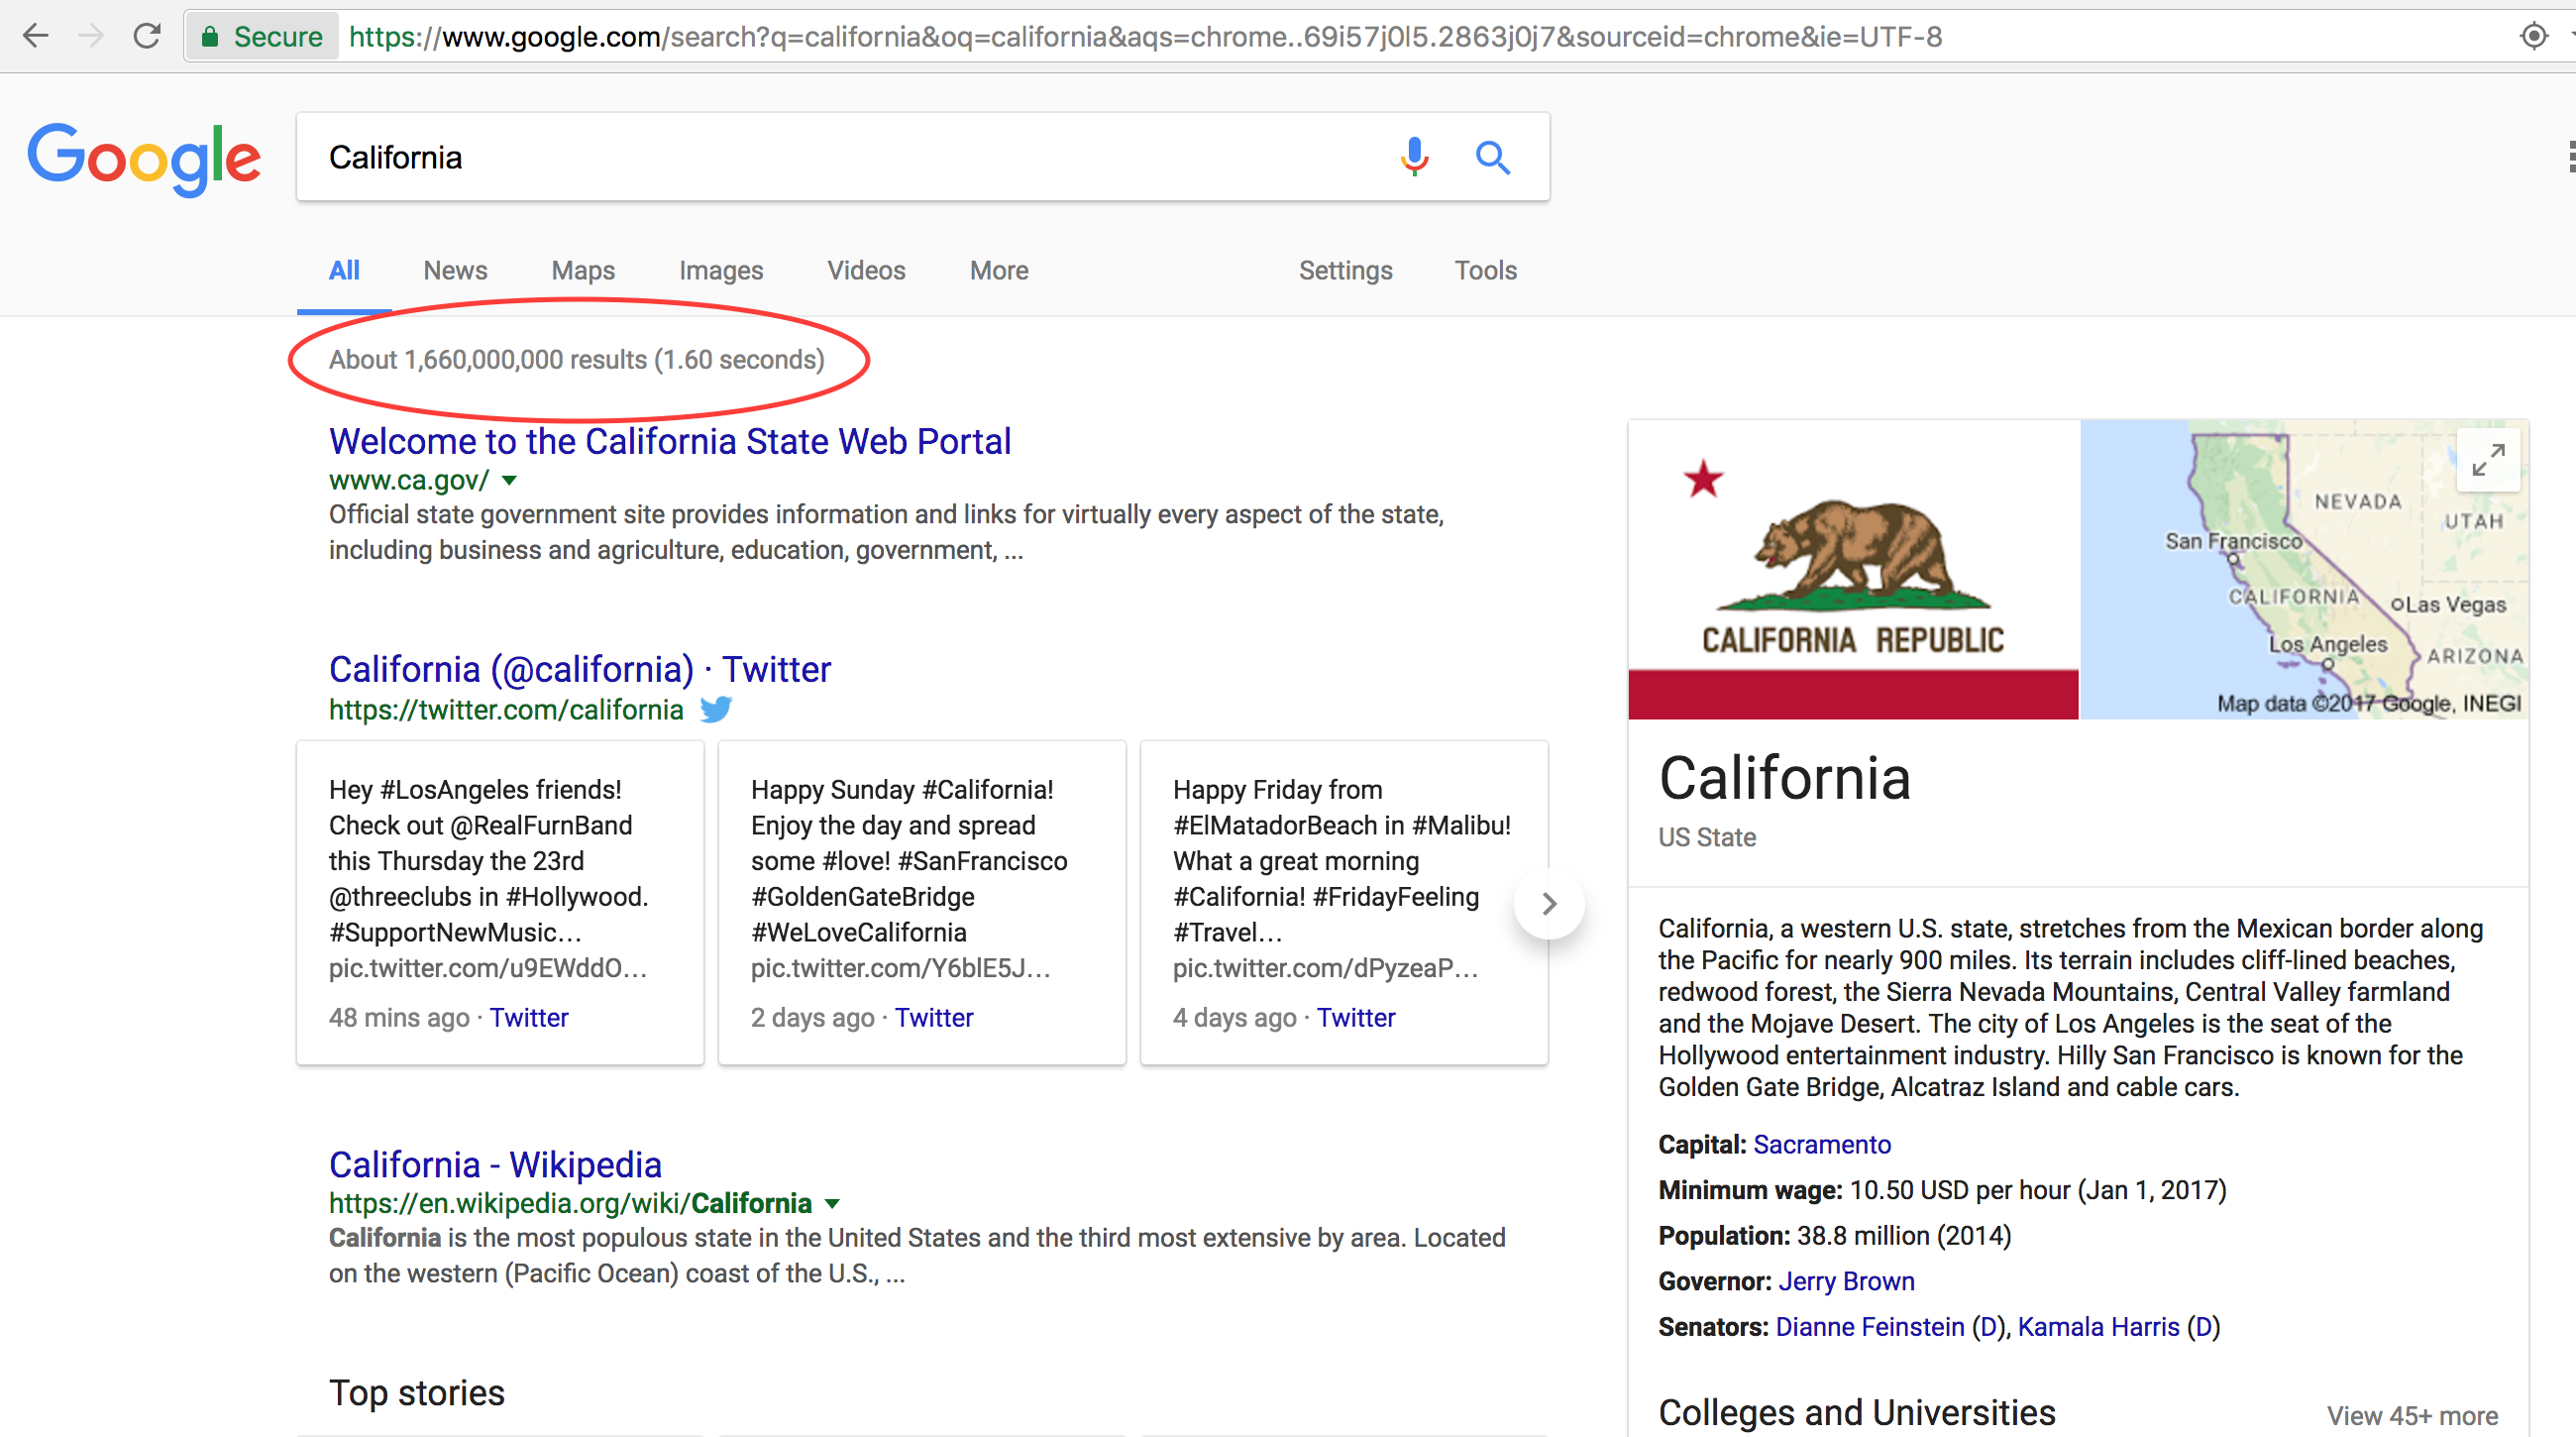
\includegraphics[scale=0.33]{idfDocsTerm.png}
\caption{Results from Google query of \emph{California}}
\label{fig:q2cali}
\end{figure}


\begin{table}
\begin{tabular}{ | l | l | l | p{7.8cm} | }
\hline
\textbf{TFIDF} & \textbf{TF} & \textbf{IDF} & \textbf{URI} \\
\hline
0.00741 & 0.00150 & 4.9412 & \url{https://www.youtube.com/watch?v=_6mtcKN1o-E} \\
\hline
0.00276 & 0.00056 & 4.9412 & \url{http://www.patheos.com/blogs/poptheology/2017/01/shuffled-selections-january-22-28/?utm_campaign=shareaholic&utm_medium=twitter&utm_source=socialnetwork} \\
\hline
0.00380 & 0.00077 & 4.9412 & \url{http://www.lapetitemortgallery.com/nyc-artist-james-brown-drawing/} \\
\hline
0.00143 & 0.00029 & 4.9412 & \url{http://www.newslocker.com/en-us/music/r-and-b-hip-hop-news/see-this-amazing-nj-teen-blend-hop-hop-jazz-and-rampb-on-youtube-njcom/} \\
\hline
0.00642 & 0.00130 & 4.9412 & \url{https://www.youtube.com/watch?v=jbe_1sNGQ2o} \\
\hline
0.00424 & 0.00086 & 4.9412 & \url{http://www.lctmag.com/operations/news/719804/empirecls-adds-mci-luxury-buses-with-3-point-seatbelts?utm_source=dlvr.it&utm_medium=twitter} \\
\hline
0.00400 & 0.00081 & 4.9412 & \url{https://www.talkbass.com/threads/fender-marcus-miller-mij-jazz-with-j-east-preamp.1266114/?utm_source=dlvr.it&utm_medium=twitter} \\
\hline
0.00168 & 0.00034 & 4.9412 & \url{https://www.theatlantic.com/entertainment/archive/2017/01/missy-elliott-im-better-jamiroquai-automaton-videos/514736/?utm_source=twb} \\
\hline
0.00434 & 0.00088 & 4.9412 & \url{http://thesop.org/story/20170131/judyth-piazza-interviews-renowned-jazz-vocalist-jan-daley.html} \\
\hline
0.00889 & 0.00180 & 4.9412 & \url{https://www.youtube.com/watch?v=C7uYx1J0hzU} \\
\hline
\end{tabular}
\caption{10 URIs found containing \emph{California}, with calculations TFIDF, TF and IDF}
\label{table:tfidf}
\end{table}

\clearpage

% =================================
% Third question
% =================================

\section*{3}

\subsection*{Question}

\begin{verbatim}
3.  Now rank the same 10 URIs from question #2, but this time 
by their PageRank.  Use any of the free PR estimaters on the web,
such as:

http://pr.eyedomain.com/
http://www.prchecker.info/check_page_rank.php
http://www.seocentro.com/tools/search-engines/pagerank.html
http://www.checkpagerank.net/

If you use these tools, you'll have to do so by hand (they have
anti-bot captchas), but there are only 10 to do.  Normalize the
values they give you to be from 0 to 1.0.  Use the same tool on all
10 (again, consistency is more important than accuracy).  Also
note that these tools typically report on the domain rather than
the page, so it's not entirely accurate.  

Create a table similar to Table 1:

Table 2.  10 hits for the term "shadow", ranked by PageRank.

PageRank	URI
--------	---
0.9		http://bar.com/
0.5		http://foo.com/

Briefly compare and contrast the rankings produced in questions 2
and 3.
\end{verbatim}

\clearpage
\subsection*{Answer}

Using the \url{pr.eyedomain.com} website I checked the page rank of my 10 URIs obtained from question 2 \cite{eyedomainref}. This website only did domain searches on the URIs provided, making the 3 youtube URIs included the same value for each Page Rank. I attempted to use the seocentro page rank but it was prompting me to pay after 3 attempts so I stuck with \url{pr.eyeomdain.com}. I also attempted prchecker.info and checkerpagerank.net but was unable to get past their captchas. The end result is shown in Table \ref{table:pgrank}.

When comparing the Page Rank to the TFIDF for each of the URIs, it's apparent that Page Rank is a much higher value for each of the URIs. What was surprising to me was the difference in TFIDF but also the values of the youtube URIs. The youtube URIs tend to correlate as the top 3 highest TFIDF values as well as the top Page Rank values.  The terms and the TFIDF for majority of the values actually correlates very nicely with one another. However the biggest discrepancy was the Page Rank and TFIDF for theatlantic.com. The Page Rank of theatlantic.com was 0.8 but it also had the second lowest TFIDF. Upon visiting the website personally I searched for my query term \emph{California} only to find it in a dropdown on the page showing that TFIDF isn't as reliable compared to Page Rank. This URI turned out to be a very high indexed news website, but TFIDF wasn't reliable enough to receive great values on this URI.

\begin{table}
\begin{tabular}{ | l | l | p{8.2cm} | }
\hline
\textbf{PR} & \textbf{TFIDF} & \textbf{URI} \\
\hline
0.9 &  0.00741 & \url{https://www.youtube.com/watch?v=_6mtcKN1o-E} \\
\hline
0.6 & 0.00276 & \url{http://www.patheos.com/blogs/poptheology/2017/01/shuffled-selections-january-22-28/?utm_campaign=shareaholic&utm_medium=twitter&utm_source=socialnetwork} \\
\hline
0.4 & 0.00380 & \url{http://www.lapetitemortgallery.com/nyc-artist-james-brown-drawing/} \\
\hline
0.2 & 0.00143 & \url{http://www.newslocker.com/en-us/music/r-and-b-hip-hop-news/see-this-amazing-nj-teen-blend-hop-hop-jazz-and-rampb-on-youtube-njcom/} \\
\hline
0.9 & 0.00642 & \url{https://www.youtube.com/watch?v=jbe_1sNGQ2o} \\
\hline
0.5 & 0.00424 & \url{http://www.lctmag.com/operations/news/719804/empirecls-adds-mci-luxury-buses-with-3-point-seatbelts?utm_source=dlvr.it&utm_medium=twitter} \\
\hline
0.4 & 0.00400 & \url{https://www.talkbass.com/threads/fender-marcus-miller-mij-jazz-with-j-east-preamp.1266114/?utm_source=dlvr.it&utm_medium=twitter} \\
\hline
0.8 & 0.00168 & \url{https://www.theatlantic.com/entertainment/archive/2017/01/missy-elliott-im-better-jamiroquai-automaton-videos/514736/?utm_source=twb} \\
\hline
0.4 & 0.00434 & \url{http://thesop.org/story/20170131/judyth-piazza-interviews-renowned-jazz-vocalist-jan-daley.html} \\
\hline
0.9 & 0.00889 & \url{https://www.youtube.com/watch?v=C7uYx1J0hzU} \\
\hline
\end{tabular}
\caption{Page Rank and TFIDF Comparison of 10 URIs with PR on a 0 to 1 scale}
\label{table:pgrank}
\end{table}

\clearpage

% =================================
% Extra Credit 1
% =================================

\section*{4}

\subsection*{Question}

\begin{verbatim}
====================================================
======Question 4 is for 3 points extra credit=======
====================================================

4.  Compute the Kendall Tau_b score for both lists (use "b" because
there will likely be tie values in the rankings).  Report both the
Tau value and the "p" value.

See: 
http://stackoverflow.com/questions/2557863/measures-
of-association-in-r-kendalls-tau-b-and-tau-c
http://en.wikipedia.org/wiki/Kendall_tau_rank_correlation_coefficient#Tau-b
http://en.wikipedia.org/wiki/Correlation_and_dependence
\end{verbatim}

\clearpage
\subsection*{Answer}

Approaching this problem I had little knowledge of what the purpose of the Kendall $Tau_b$ score. Although I still feel uneasy about a few parts of the equation, as shown below, I felt I got a general knowledge of what its result yields. The following Kendall $Tau_b$ equation was taken from Wikipedia \cite{wikipediaref}.

\[ \tau_b = \frac{n_c - n_d}{\sqrt{(n_0 - n_1)(n_0 - n_2)}} \]

where

\[ n_0 = n(n-1)/2 \]
\[ n_1 = \sum_i t_i (t_i - 1)/2 \]
\[ n_2 = \sum_j u_j (u_j - 1)/2 \]
\[ n_c = \textrm{Number of concordant pairs} \]
\[ n_d = \textrm{Number of discordant pairs} \]
\[ t_i = \textrm{Number of tied values in the $i^{th}$ group of ties for the first quantity} \]
\[ u_j = \textrm{Number of tied values in the $j^{th}$ group of ties for the second quantity} \]

Basically this creates a correlation between the paired values. The $tau$ value can have a coefficient between -1 to 1. Any value less that 1, meant there is a negative correlation and that page rank is the opposite of the TFIDF value. Any value greater than 1 means that there is a positive correlation showing that the correlation between page rank and TFIDF are similar, if its at 1 it represents a perfect match. If the value is at zero or very close to zero this means that there is no correlation between the page rank and TFIDF. I stated before that I thought they actually correlated fairly well, and Dr. Nelson would say, ``That's an engineer's answer.''

Therefore using the stackoverflow post mentioned in the question, I found an R library called Kendall which computes the Kendall $Tau_b$ value \cite{stackoverflowpostref}. The code to generate this value is below in Listing \ref{lst:q4kendall}.

\lstinputlisting[frame=single,caption={R script to calculate Kendall $Tau_b$ between page rank and TFIDF from previous 10 URIs},label=lst:q4kendall,captionpos=b,numbers=left,showspaces=false,showstringspaces=false,basicstyle=\footnotesize]{\srcPath/kendall-tau.R}

The summary produced:
\begin{verbatim}
Score =  19 , Var(Score) = 117.6667
denominator =  41.89272
tau = 0.454, 2-sided pvalue =0.097039
\end{verbatim}

The tau was above 0 making it a positive correlation and also supporting my Engineer's hypothesis that it correlates.

% =================================
% Extra Credit 2
% =================================

\clearpage
\section*{5}

\subsection*{Question}

\begin{verbatim}
====================================================
======Question 7 is for 2 points extra credit=======
====================================================

7.  Build a simple (i.e., no positional information) inverted file
(in ASCII) for all the words from your 1000 URIs.  Upload the entire
file to github and discuss an interesting portion of the file in
your report.
\end{verbatim}

\clearpage
\subsection*{Answer}

To complete this question I decided not to create write my own code but base it off a sample code provided on Rosetta Code as shown in Listing \ref{lst:q7inverted}, named \textbf{simpleInvertedIndex.py} \cite{invertedindexref}. It first goes through each processed file splitting the words and associates words with that file. After going through all 1000 processed files it would then sort each word found in any of those files and associate the word with all related the files in a key pair association, where the value was an array of the text files with the values.

This lead to some very interesting results. The keys that were most interesting were actually numbers. It was found that single character, single digit, were in the most files. This also seemed to be true for any single character in a document, such as: commas, backslashes, apostrophes, question marks, etc. As the key term was getting larger in total characters, it tended to have less and less file associations. Which to me makes sense as a majority of words in the english language don't have to cross six characters.

Years also seemed to be a great find in this inverted index. I found years starting from 2010 up to 2017, there could be more, that also had multiple occurrences in files. Older years seemed less prevalent in these documents. I found that each year after 2010 slightly went up in number of appearances in files, while 2017 at the end had the most number of occurrences.

Finally the emojis had game in these documents, but were fairly scarce but some managed to appear a in a few documents as shown in Figure \ref{fig:q7emojis}.

\lstinputlisting[frame=single,caption={Python script to create an inverted index},label=lst:q7inverted,captionpos=b,numbers=left,showspaces=false,showstringspaces=false,basicstyle=\footnotesize]{\srcPath/simpleInvertedIndex.py}

\begin{figure}[h]
\centering
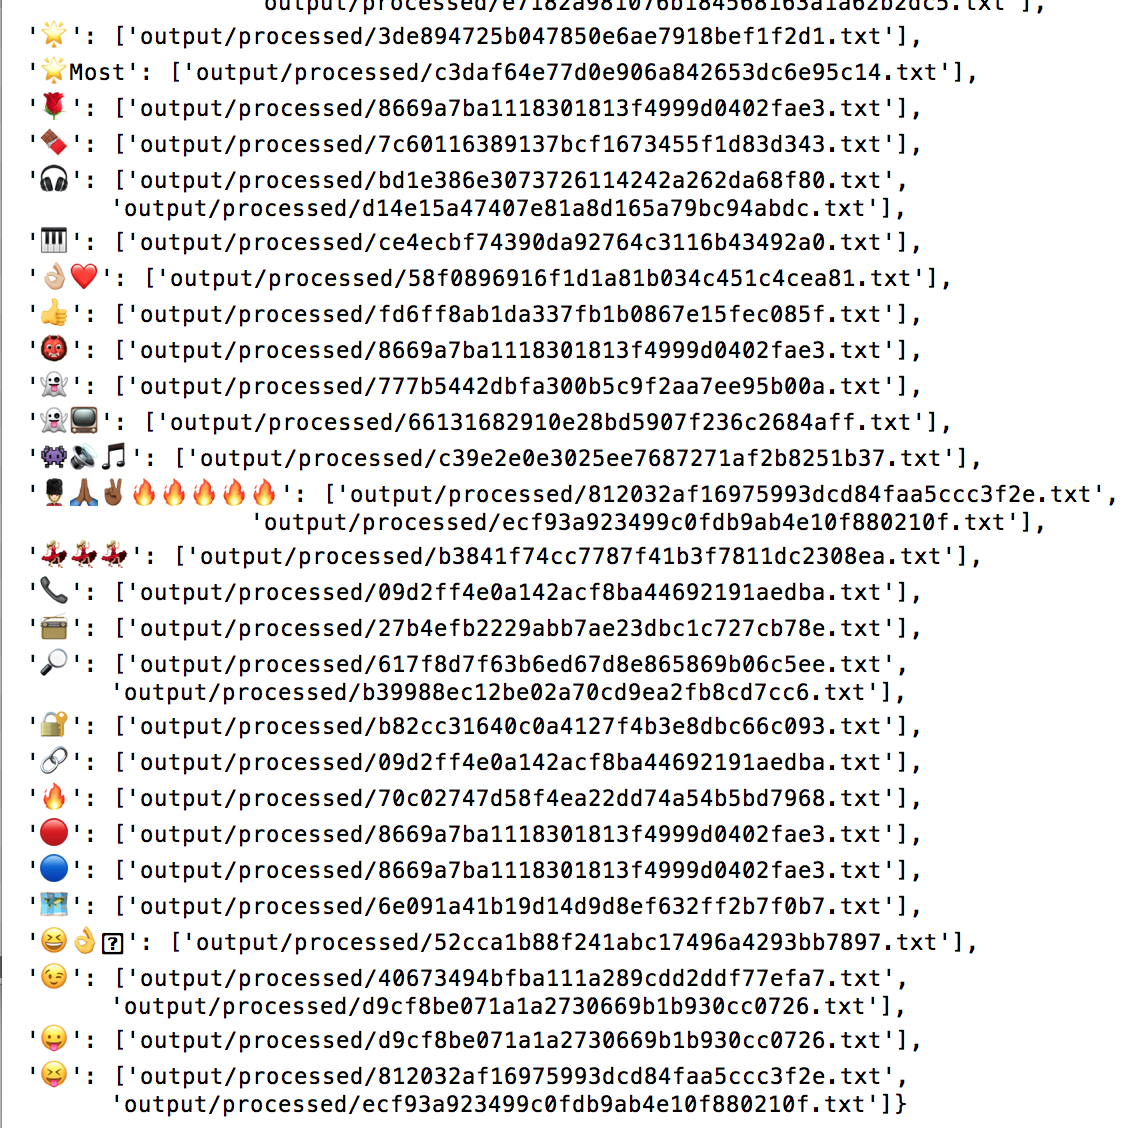
\includegraphics[scale=0.65]{emojiIndex.png}
\caption{Inverted Index emojis found}
\label{fig:q7emojis}
\end{figure}


\clearpage
% =================================
% Bibliography
% =================================

\begin{thebibliography}{9}
\bibitem{eyedomainref}
``Check last known Google PageRank.'' eyedomain. EyeDomain, n.d. Web. 22 Feb. 2017. \url{http://pr.eyedomain.com/}.
\bibitem{invertedindexref}
``Inverted Index.'' Roseta Code Inverted index. N.p.,n.d. Web. 22 Feb. 2017. \url{http://rosettacode.org/wiki/Inverted_index#Simple_inverted_index}
\bibitem{wikipediaref}
``Kendall rank correlation coefficient.'' Wikipedia - Kendall Rank Correlation coefficient. Wikipedia, n.d. Web. 22 Feb. 2017. \url{https://en.wikipedia.org/wiki/Kendall_rank_correlation_coefficient#Tau-b}
\bibitem{finalurisref}
Atkins, Grant. ``finalURIs.txt - Twitter scraped URIs.'' cs532-s17 Github Repository. N.p., 09 Feb. 2017. Web. 22 Feb. 2017.\url{https://github.com/grantat/cs532-s17/blob/master/assignments/A3/src/output/finalURIs.txt}.
\bibitem{finalurisref}
Atkins, Grant. ``Inverted Index results.'' cs532-s17 Github Repository. N.p., 09 Feb. 2017. Web. 22 Feb. 2017.\url{https://github.com/grantat/cs532-s17/blob/master/assignments/A3/src/output/invertedIndex.txt}.
\bibitem{stackoverflowpostref}
Fellows, Ian. ``Measures of association in R ? Kendall's tau-b and tau-c.'' Stackoverflow. Stackoverflow, 10 April 2010. Web. 22 Feb. 2017. \url{http://stackoverflow.com/questions/2557863/measures-of-association-in-r-kendalls-tau-b-and-tau-c}.
\bibitem{worldwidewebsizeref}
Kunder, Maurice. ``The size of the Dutch World Wide Web'' worldwidwebsize. N.p., n.d. Web. 22 Feb. 2017.\url{http://www.worldwidewebsize.com/}.
\bibitem{curlref} 
Stenberg, Daniel. ``Curl.1 the Man Page.'' Curl - How To Use. N.p., n.d. Web. 24 Jan. 2017. \url{https://curl.haxx.se/docs/manpage.html}.
\end{thebibliography}

\end{document}